% vim: set spell spelllang=en tw=100 et sw=4 sts=4 foldmethod=marker foldmarker={{{,}}} :

\documentclass{beamer}

\usepackage{xcolor}
\usepackage{hyperref}
\usepackage{tikz}
\usepackage{microtype}
\usepackage{amsmath}
\usepackage{amsfonts}
\usepackage{amssymb}
\usepackage{listings}
\usepackage{csquotes}
\usepackage{fancyvrb}
\usepackage{bussproofs}
\usepackage{booktabs}
\usepackage{bigstrut}
\usepackage{xspace}
\usepackage{mathtools}
\usepackage{pifont}

\RequirePackage[tt=false, type1=true]{libertine}
\RequirePackage[varqu]{zi4}
\RequirePackage[libertine]{newtxmath}
\RequirePackage[T1]{fontenc}

\usetikzlibrary{shapes, arrows, shadows, calc, positioning, fit,
    decorations.pathreplacing, decorations.pathmorphing, shapes.misc,
    tikzmark, backgrounds, trees, overlay-beamer-styles}

\definecolor{uofguniversityblue}{rgb}{0, 0.219608, 0.396078}
\definecolor{uofgheather}{rgb}{0.356863, 0.32549, 0.490196}
\definecolor{uofgaquamarine}{rgb}{0.603922, 0.72549, 0.678431}
\definecolor{uofgslate}{rgb}{0.309804, 0.34902, 0.380392}
\definecolor{uofgrose}{rgb}{0.823529, 0.470588, 0.709804}
\definecolor{uofgmocha}{rgb}{0.709804, 0.564706, 0.47451}
\definecolor{uofgsandstone}{rgb}{0.321569, 0.278431, 0.231373}
\definecolor{uofgforest}{rgb}{0, 0.2, 0.129412}
\definecolor{uofglawn}{rgb}{0.517647, 0.741176, 0}
\definecolor{uofgcobalt}{rgb}{0, 0.615686, 0.92549}
\definecolor{uofgturquoise}{rgb}{0, 0.709804, 0.819608}
\definecolor{uofgsunshine}{rgb}{1.0, 0.862745, 0.211765}
\definecolor{uofgpumpkin}{rgb}{1.0, 0.72549, 0.282353}
\definecolor{uofgthistle}{rgb}{0.584314, 0.070588, 0.447059}
\definecolor{uofgrust}{rgb}{0.603922, 0.227451, 0.023529}
\definecolor{uofgburgundy}{rgb}{0.490196, 0.133333, 0.223529}
\definecolor{uofgpillarbox}{rgb}{0.701961, 0.047059, 0}
\definecolor{uofglavendar}{rgb}{0.356863, 0.301961, 0.580392}

\newcommand*{\rom}[1]{\emph{\romannumeral #1 \relax}}
\newcommand{\neighbourhood}{\operatorname{N}}
\newcommand{\vertexset}{\operatorname{V}}
\newcommand{\degree}{\operatorname{deg}}

% Pseudo-Boolean constraints
\newcommand{\coeffa}{a}
\newcommand{\coeffb}{b}
\newcommand{\coeffc}{c}
\newcommand{\coeffd}{d}
\newcommand{\coeffk}{k}
\newcommand{\coeffw}{w}
\newcommand{\consta}{A}
\newcommand{\constb}{B}
\newcommand{\constk}{k}
\newcommand{\constw}{W}
\newcommand{\litell}{\ell}
\newcommand{\factor}{c}
\newcommand{\monomm}{m}
\newcommand{\degd}{d}
\newcommand{\lita}{\ensuremath{a}}
\newcommand{\litb}{\ensuremath{b}}
\newcommand{\litc}{\ensuremath{c}}
\newcommand{\litd}{\ensuremath{d}}
\newcommand{\litl}{\ensuremath{\ell}}
\newcommand{\formf}{F}
\newcommand{\constrc}{C}
\newcommand{\clc}{\ensuremath{C}}
\newcommand{\wrt}{with respect to\xspace}
\newcommand{\objf}{f}
\newcommand{\tvastd}{{\ensuremath{\alpha}}}

\newcommand{\pbdeg}[1]{\numfuncformat{deg}(#1)}

\newcommand{\pbrelation}{\bowtie}

\newcommand{\Lor}{\bigvee}
\newcommand{\Land}{\bigwedge}

\newcommand{\pbconstra}{\textstyle \sum_i \coeffa_i \litell_i \geq \consta}
\newcommand{\pbconstrb}{\textstyle \sum_i \coeffb_i \litell_i \geq \constb}
% Use \pbconstrlincomb with arguments i, a, A, b, B c_a c_b
\newcommand{\pbconstrlincomb}[7]%
    {\textstyle \sum_{#1}
      ({#6} {#2}_{#1} + {#7}{#4}_{#1}) \litell_{#1} 
      \geq
      {#6} {#3} + {#7}{#5}}

\newcommand{\Z}{\mathbb{Z}}
\newcommand{\N}{\mathbb{N}}
\newcommand{\Nplus}{\mathbb{N}^{+}}
\newcommand{\Nzero}{\mathbb{N}_{0}}
\newcommand{\varx}{\ensuremath{x}}
\newcommand{\vara}{a}
\newcommand{\varb}{b}
\newcommand{\olnot}[1]{\overline{#1}}
\newcommand{\derivruleformat}[1]{\textcolor{uofgcobalt}{\textbf{#1}}\xspace}
\newcommand{\langstd}{\ensuremath{L}}

\newcommand{\ceiling}[1]{\lceil #1 \rceil}
\newcommand{\Ceiling}[1]{\bigl \lceil #1 \bigr \rceil}
\newcommand{\CEILING}[1]{\left \lceil #1 \right \rceil}

\newcommand{\restrict}[2]{#1_{\upharpoonright#2}}

\newcommand{\limpl}{\rightarrow}
\newcommand{\lequiv}{\leftrightarrow}
\newcommand{\lortight}{\!\lor\!}
\newcommand{\set}[1]{\{ #1 \}}
\newcommand{\setsize}[1]{{\left|#1\right|}}

\newcommand{\solvernameformat}[1]{\emph{#1}}
\newcommand{\CryptoMiniSat}{\solvernameformat{CryptoMiniSat}\xspace}

\newcommand{\proofsystemformat}[1]{\textsc{#1}\@}
\newcommand{\drat}{\proofsystemformat{DRAT}\xspace}
\newcommand{\frat}{\proofsystemformat{FRAT}\xspace}
\newcommand{\grit}{\proofsystemformat{GRIT}\xspace}
\newcommand{\lrat}{\proofsystemformat{LRAT}\xspace}

\newcommand{\toolformat}[1]{\textit{#1}}
\newcommand{\veripb}{\toolformat{VeriPB}\xspace}

\newcommand{\emptycl}{\bot}

% {{{ theme things
\useoutertheme[footline=authortitle]{miniframes}
\useinnertheme{rectangles}

\setbeamerfont{block title}{size={}}
\setbeamerfont{title}{size=\large,series=\bfseries}
\setbeamerfont{section title}{size=\large,series=\mdseries}
\setbeamerfont{author}{size=\normalsize,series=\mdseries}
\setbeamercolor*{structure}{fg=uofguniversityblue}
\setbeamercolor*{palette primary}{use=structure,fg=black,bg=white}
\setbeamercolor*{palette secondary}{use=structure,fg=white,bg=uofgcobalt}
\setbeamercolor*{palette tertiary}{use=structure,fg=white,bg=uofguniversityblue}
\setbeamercolor*{palette quaternary}{fg=white,bg=black}
\setbeamercolor{block body}{bg=structure!10}
\setbeamercolor{block title}{bg=structure,fg=white}
\setbeamertemplate{blocks}[rounded]
\setbeamercolor*{titlelike}{parent=palette primary}

% Some settings for getting a bibliography that doesn't take up too much space
\setbeamertemplate{bibliography entry title}{}
\setbeamertemplate{bibliography entry location}{}
\setbeamertemplate{bibliography entry note}{}

% Get usual references in bibliography, not icons
\setbeamertemplate{bibliography item}[text]

\beamertemplatenavigationsymbolsempty

\setbeamertemplate{title page}
{
    \begin{tikzpicture}[remember picture, overlay]
        \node at (current page.north west) {
            \begin{tikzpicture}[remember picture, overlay]
                \fill [fill=uofguniversityblue, anchor=north west] (0, 0) rectangle (\paperwidth, -2.8cm);
            \end{tikzpicture}
        };

        \node (logo) [anchor=north east, shift={(-0.6cm,-0.3cm)}] at (current page.north east) {
            
\includegraphics[keepaspectratio=true,scale=0.5]{UoG_keyline.pdf}
        };

        \node (logo2) [anchor=north, below=0.03cm of logo.south] {
            
\includegraphics[keepaspectratio=true,scale=0.1]{RAEngWhite.pdf}
        };

        \coordinate (logos) at ($(logo.south)!0.5!(logo2.north)$);

        \node [anchor=west, xshift=0.2cm] at (current page.west |- logos) {
            \begin{minipage}{0.5\paperwidth}\raggedright
                {\usebeamerfont{title}\usebeamercolor[white]{}\inserttitle}\\[0.1cm]
                {\usebeamerfont{author}\usebeamercolor[white]{}\insertauthor}\\[0.1cm]
            \end{minipage}
        };
    \end{tikzpicture}
}

\newcommand{\frameofframes}{/}
\newcommand{\setframeofframes}[1]{\renewcommand{\frameofframes}{#1}}

\makeatletter
\setbeamertemplate{footline}
{%
    \begin{beamercolorbox}[colsep=1.5pt]{upper separation line foot}
    \end{beamercolorbox}
    \begin{beamercolorbox}[ht=2.5ex,dp=1.125ex,%
        leftskip=.3cm,rightskip=.3cm plus1fil]{author in head/foot}%
        \leavevmode{\usebeamerfont{author in head/foot}\insertshortauthor}%
        \hfill%
        {\usebeamerfont{institute in head/foot}\usebeamercolor[fg]{institute in head/foot}\insertshortinstitute}%
    \end{beamercolorbox}%
    \begin{beamercolorbox}[ht=2.5ex,dp=1.125ex,%
        leftskip=.3cm,rightskip=.3cm plus1fil]{title in head/foot}%
        {\usebeamerfont{title in head/foot}\insertshorttitle}%
        \hfill%
        {\usebeamerfont{frame number}\usebeamercolor[fg]{frame number}\insertframenumber~\frameofframes~\inserttotalframenumber}
    \end{beamercolorbox}%
    \begin{beamercolorbox}[colsep=1.5pt]{lower separation line foot}
    \end{beamercolorbox}
}

\makeatletter
\newenvironment{nearlyplainframe}[2][]{
    \def\beamer@entrycode{\vspace*{-\headheight}\vspace*{3pt}}
    \setbeamertemplate{headline}
    {%
        \begin{beamercolorbox}[colsep=1.5pt]{upper separation line head}
        \end{beamercolorbox}
        \begin{beamercolorbox}[ht=0.5ex,dp=0.125ex,%
            leftskip=.3cm,rightskip=.3cm plus1fil]{title in head/foot}%
        \end{beamercolorbox}%
        \begin{beamercolorbox}[ht=0.5ex,dp=0.125ex,%
            leftskip=.3cm,rightskip=.3cm plus1fil]{author in head/foot}%
        \end{beamercolorbox}%
        \begin{beamercolorbox}[colsep=1.5pt]{lower separation line head}
        \end{beamercolorbox}
        \vspace*{\headheight}
    }

    \setbeamertemplate{footline}
    {%
        \begin{beamercolorbox}[colsep=1.5pt]{upper separation line foot}
        \end{beamercolorbox}
        \begin{beamercolorbox}[ht=0.5ex,dp=0.125ex,%
            leftskip=.3cm,rightskip=.3cm plus1fil]{author in head/foot}%
        \end{beamercolorbox}%
        \begin{beamercolorbox}[ht=0.5ex,dp=0.125ex,%
            leftskip=.3cm,rightskip=.3cm plus1fil]{title in head/foot}%
        \end{beamercolorbox}%
        \begin{beamercolorbox}[colsep=1.5pt]{lower separation line foot}
        \end{beamercolorbox}
    }

    \begin{frame}[#1]{#2}
    }{
    \end{frame}
}
\makeatother

% }}}

\author{Ciaran McCreesh}
\title{Proof Logging}

\begin{document}

{
    \usebackgroundtemplate{
        \tikz[overlay, remember picture]
        \node[at=(current page.south), anchor=south, inner sep=0pt, yshift=-0.7cm]{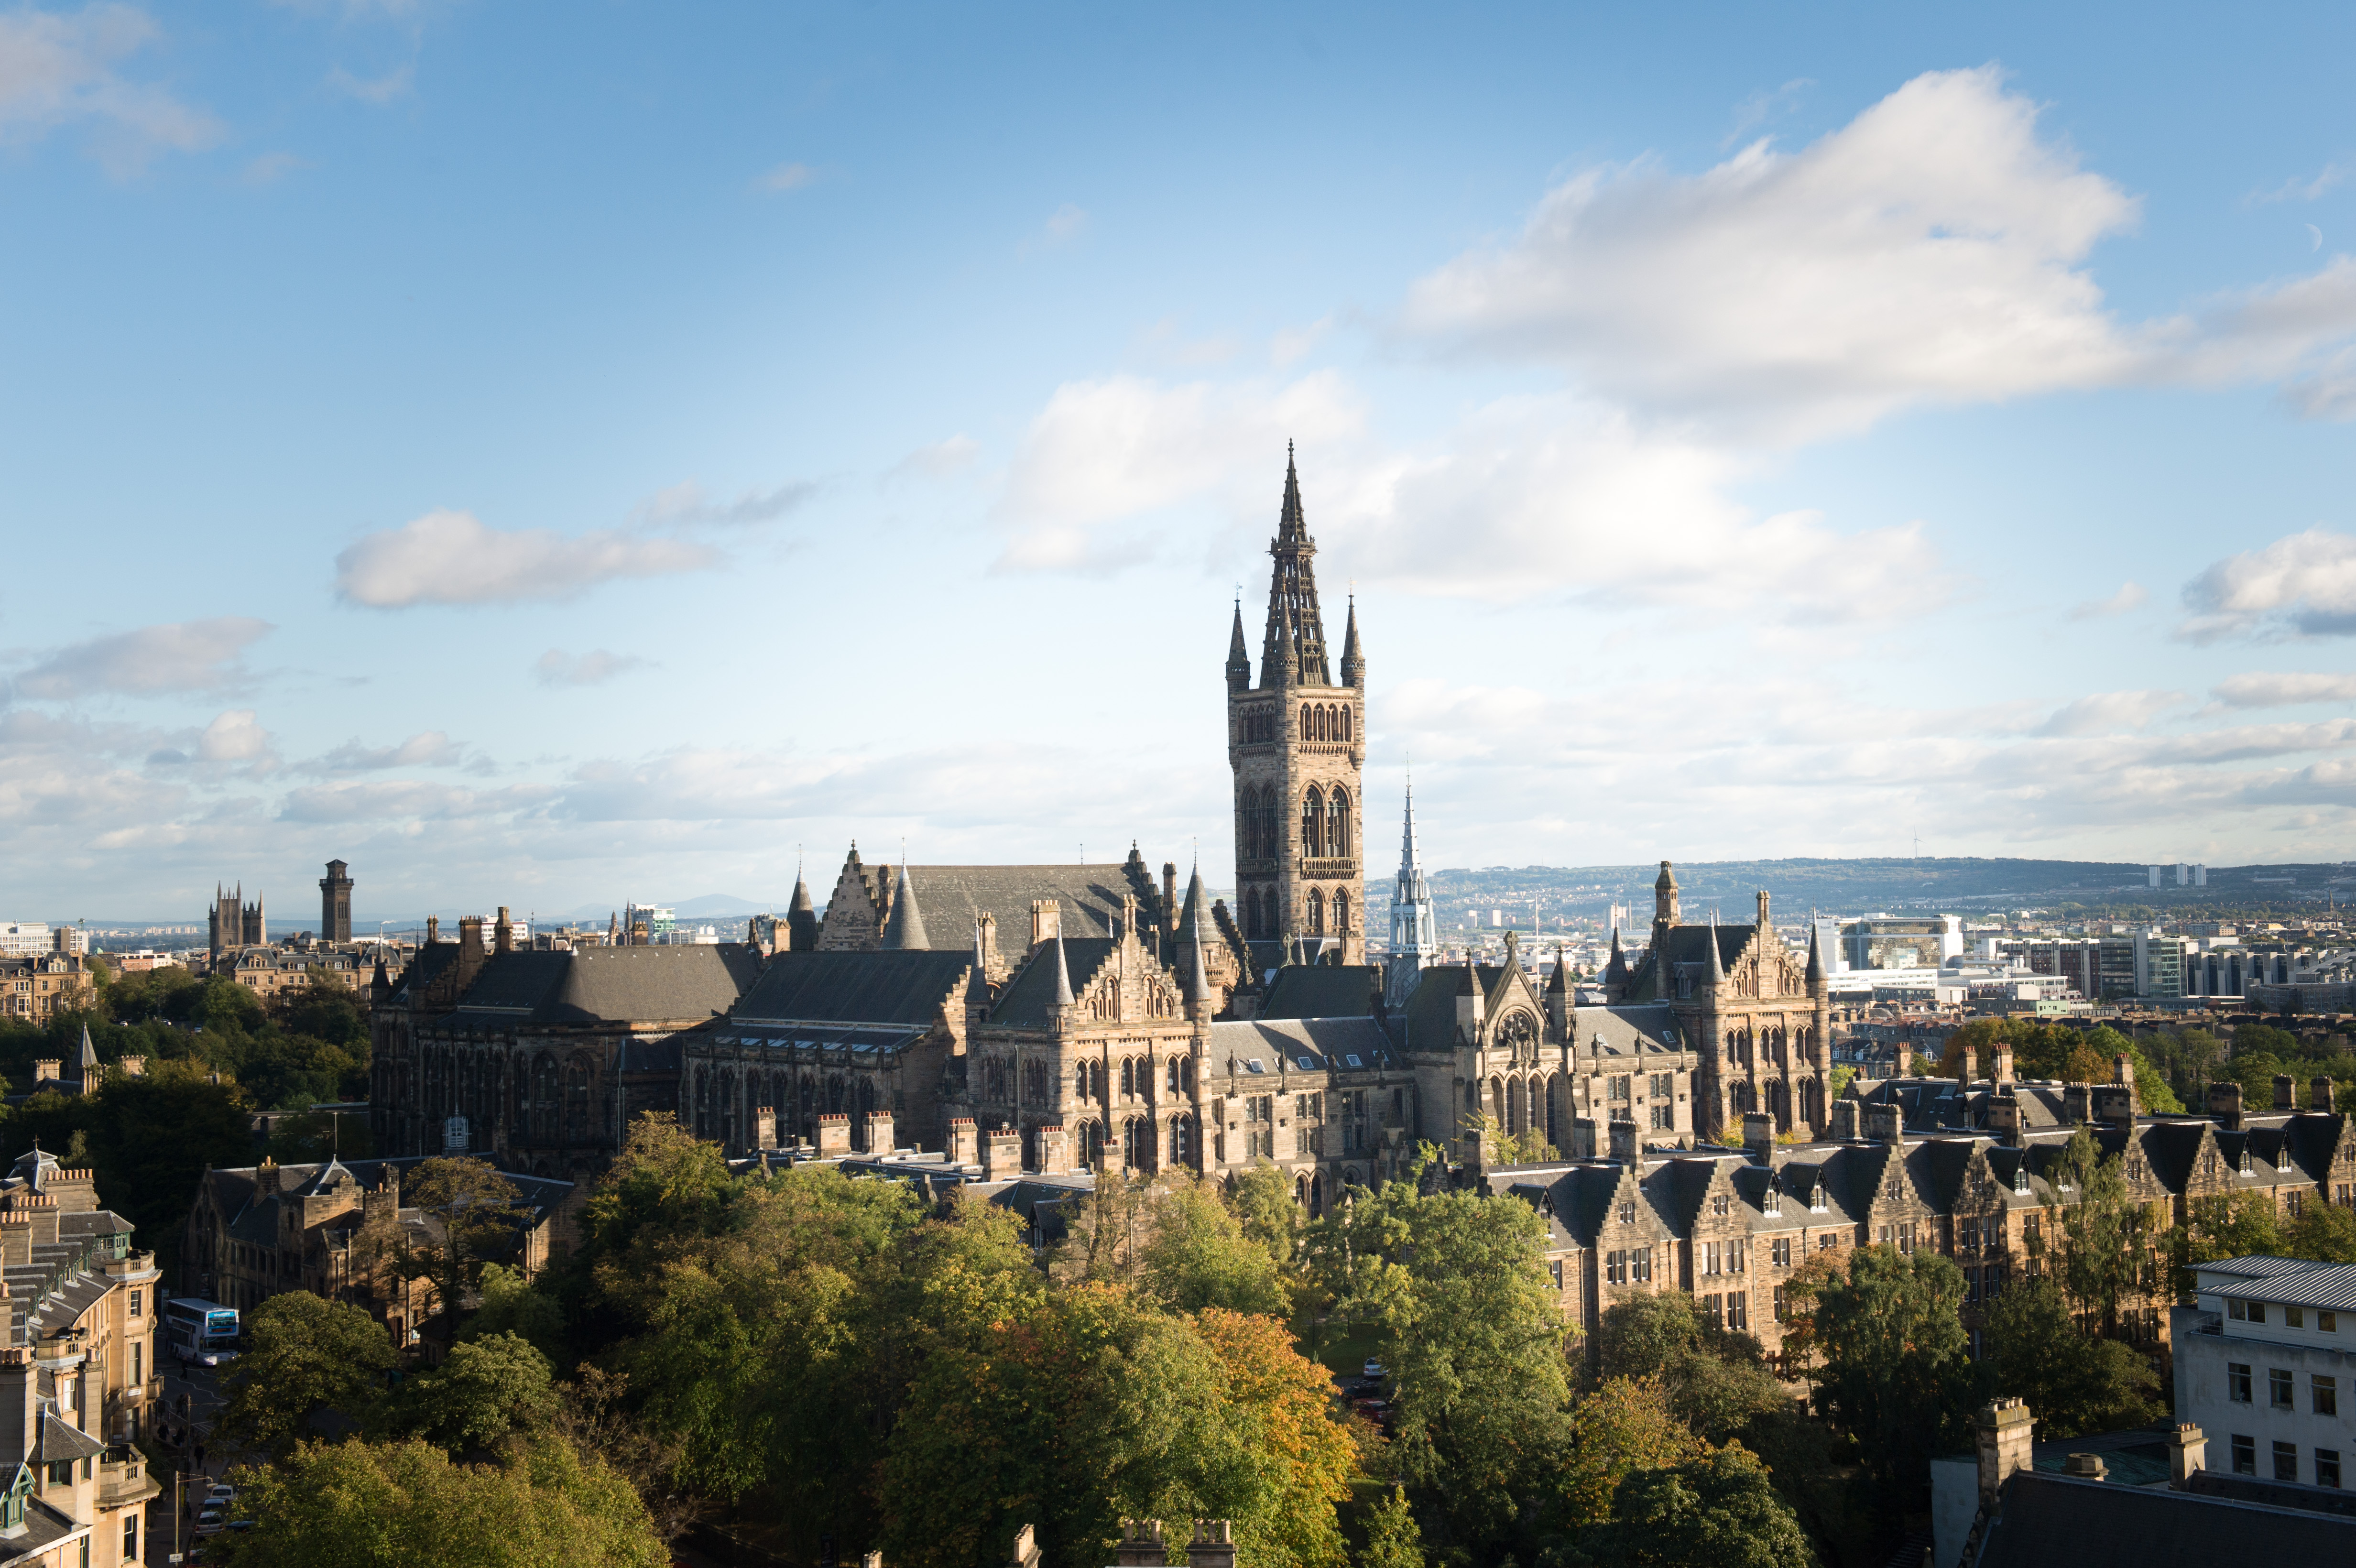
\includegraphics[keepaspectratio=true, height=\paperheight]{background5.jpg}};
    }
    \begin{frame}[plain,noframenumbering]
        \titlepage
    \end{frame}
}

\begin{frame}{Demotivation}
    My first experience of research: a summer internship reimplementing a clique algorithm from the literature.

    \bigskip

    My code produced the ``wrong'' answer on a few instances.

    \bigskip\pause

    I spent a month trying to find and fix it.

    \bigskip\pause

    The published answers were wrong.
\end{frame}

\begin{frame}{How Do We Know Our Solvers Are Correct?}
    I've wanted to write a CP solver for years.

    \bigskip

    How will I know it's right? What if I ruin some poor student's life by publishing wrong answers?

    \bigskip\pause

    What if someone uses my solver for kidney exchange or workplace allocation or deciding adoptive parents?
\end{frame}

\begin{frame}{The Slide That ``They'' Don't Want Me to Show You}
    The 2021 MiniZinc challenge: for 1.28\% of instances, wrong solutions were claimed.
    \\
    \begin{itemize}
        \item False claims of unsatisfiability.
        \item False claims of optimality.
        \item Infeasible solutions produced.
        \item Not limited to a single solver, problem, or constraint.
        \item Not even consistent---same solver on same hardware and same instance can give
            different results on different runs.
    \end{itemize}
    \bigskip
    I don't want my solver to produce wrong answers!

    \bigskip\pause

    Or at least, when it's wrong, I want a guaranteed way of detecting it.
\end{frame}

\begin{frame}{Testing?}
    \only<1>{\begin{itemize}
        \item Traditional software engineering testing techniques only catch shallow bugs.
        \item Basically useless for complicated algorithms\ldots
        \item We do have special ways of testing constraint solvers.
    \end{itemize}}
    \only<2>{
        \centering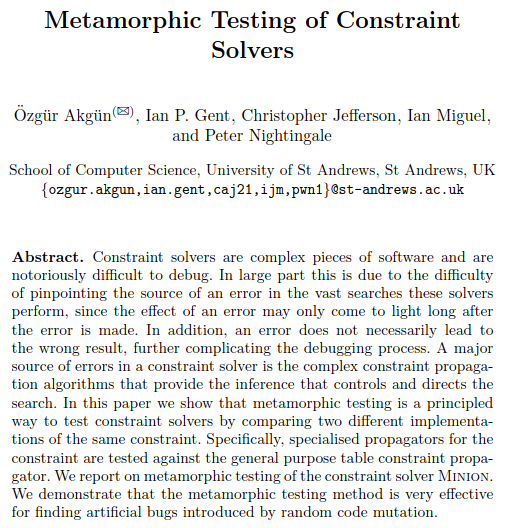
\includegraphics[keepaspectratio=true,scale=0.35]{testing1.png}
    }
    \only<3>{
        \centering
\includegraphics[keepaspectratio=true,scale=0.35]{testing2.png}
    }
    \only<4>{
        \centering ``It is now two decades since it was pointed out that program testing
        may convincingly demonstrate the presence of bugs, but can never
        demonstrate their absence. After quoting this well-publicized remark
        devoutly, the software engineer returns to the order of the day and
        continues to refine his testing strategies, just like the alchemist of
        yore, who continued to refine his chrysocosmic purifications.''

        \flushright -- Edsger W. Dijkstra\\``On the cruelty of really teaching computing science''}
\end{frame}

\begin{frame}{Formal Methods / Correct By Construction Software}
    \begin{itemize}
        \item Can't even do a bad implementation of all-different yet\ldots
        \item The fast unit propagation for SAT is also beyond the reach of
            formal methods.
    \end{itemize}
\end{frame}

\begin{frame}{Another Option?}
    \begin{itemize}
        \item Idea: maybe checking that an answer is right is simpler than
            checking an algorithm?
    \end{itemize}
\end{frame}

\begin{frame}{Proof Logging in SAT}
    \only<1>{\begin{itemize}
        \item Certifying algorithms:
            \begin{itemize}
                \item Must produce a proof alongside an output.
                \item Verify outputs, not solvers.
            \end{itemize}
        \item A variety of formats for SAT: \ldots, DRAT, FRAT, \ldots.
            \begin{itemize}
                \item Unsat is the hard part.
            \end{itemize}
        \item Huge success for SAT solving.
    \end{itemize}}\only<2-3>{
    \begin{center}
        \includegraphics<2>[keepaspectratio=true,scale=0.30]{shortest-math-paper.jpg}
        \includegraphics<3>[keepaspectratio=true,scale=0.65]{nature.png}
    \end{center}}
\end{frame}

\begin{frame}{SAT Proof Logging Workflow}
    \begin{center}
        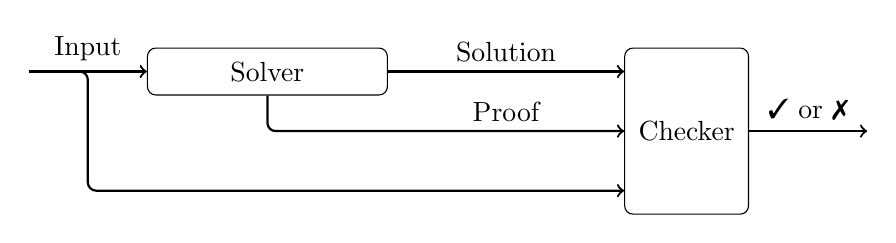
\begin{tikzpicture}
            \node (solver) [inner xsep=3em, inner ysep=0.5em, draw, rounded corners=3pt] { Solver };

            \node (checker) [right=3cm of solver.north east, anchor=north west,
            inner xsep=0.5em, draw, rounded corners=3pt, minimum height=6em, visible on=<3->] { Checker };

            \draw [->, thick] (solver.east) -- (solver.east -| checker.west)
                coordinate [midway] (solutionmid) node [above, midway] { Solution };

            \draw [->, thick, rounded corners=3pt, visible on=<2->] (solver.south) -- (solver.south |- checker.west)
                -- (checker.west) coordinate [midway] (proofmid);

            \coordinate (prooflabel) at (proofmid-|solutionmid);
            \node [above=0cm of prooflabel, visible on=<2->] { Proof };

            \coordinate [right=1.5cm of checker.east] (verified);
            \draw [->, thick, visible on=<4->] (checker.east) -- (verified) node [above, midway] { \ding{51} or \ding{55} };

            \coordinate [left=1.5cm of solver.west] (input);
            \draw [->, thick] (input) -- (solver.west) coordinate [midway] (inputmid) node [above, midway] { Input };

            \coordinate (checkerbotleft) at ($(checker.west)+($(checker.west)-(solver.east-|checker.west)$)$);

            \draw [->, thick, rounded corners=3pt, visible on=<3->] ($(inputmid)+(-0.2,0)$) -- (inputmid) -- (inputmid |- checkerbotleft) -- (checkerbotleft);
        \end{tikzpicture}
    \end{center}

  \begin{enumerate}
  \item<1->
    Run solver on problem input.
  \item<2->
    Get both a solution and a proof as output.
  \item<3->
    Feed input + solution + proof to proof checker.
  \item<4->
    Verify that proof checker says solution is correct.
  \end{enumerate}
\end{frame}

\begin{frame}{What is a Proof?}
    \begin{itemize}
        \item Start with some known facts, and some rules.
        \item Use the rules to create new facts.
        \item End up with the thing we're trying to prove.
            \begin{itemize}
                \item Rules have to be \emph{sound}.
                \item Today we're going to be talking about \emph{equisatisfiability}.
                \item Proof system has to be \emph{complete}.
            \end{itemize}
    \end{itemize}
\end{frame}

\begin{frame}{Resolution Proofs for CNF}
\only<1>{
    \begin{minipage}[c]{0.25\framewidth}
        \textcolor{uofgcobalt}{\textbf{Model axioms}}
    \end{minipage}\hfill\begin{minipage}[c]{0.70\framewidth}
        \centering From the input
    \end{minipage}\bigskip

    \begin{minipage}[c]{0.25\framewidth}
        \textcolor{uofgcobalt}{\textbf{Resolution}}
    \end{minipage}\hfill\begin{minipage}[c]{0.70\framewidth}\begin{prooftree}
        \AxiomC{$\textcolor{uofglawn}{x_1} \vee \textcolor{uofglawn}{x_2} \vee \ldots \vee
        \textcolor{uofglawn}{x_i} \vee \textcolor{uofgpillarbox}{c}$}
        \AxiomC{$\textcolor{uofgpillarbox}{\overline{c}} \vee \textcolor{uofgcobalt}{y_1} \vee
        \textcolor{uofgcobalt}{y_2} \vee \ldots \textcolor{uofgcobalt}{y_j}$}
        \BinaryInfC{$\textcolor{uofglawn}{x_1} \vee \textcolor{uofglawn}{x_2} \vee \ldots \vee
        \textcolor{uofglawn}{x_i} \vee \textcolor{uofgcobalt}{y_1} \vee
        \textcolor{uofgcobalt}{y_2} \vee \ldots \vee \textcolor{uofgcobalt}{y_j}$}
    \end{prooftree}\end{minipage}

    \bigskip

    \begin{itemize}
        \item To prove unsatisfiability: resolve until you reach the empty clause.
    \end{itemize}
}
    \only<2->{
        \begin{minipage}[c]{0.30\framewidth}
            \begin{align}
                & x \vee y \vee z \\
                & \overline{x} \vee \overline{y} \vee \overline{z} \\
                & \overline{x} \vee y \\
                & \overline{x} \vee z \\
                & x \vee \overline{y} \\
                & x \vee \overline{z}
            \end{align}
        \end{minipage}\hfill\begin{minipage}[c]{0.60\framewidth}
            \begin{align}
                & 1, 5 \operatorname{on} y && x \vee z \\
                & 6, 7 \operatorname{on} z && x \\
                & 3, 8 \operatorname{on} x && y \\
                & 4, 8 \operatorname{on} x && z \\
                & 2, 8 \operatorname{on} x && \overline{y} \vee \overline{z} \\
                & 9, 11 \operatorname{on} y && \overline{z} \\
                & 10, 12 \operatorname{on} z && \emptyset
            \end{align}

        \end{minipage}
    }
\end{frame}

\begin{frame}{Reverse Unit Propagation (RUP) Proofs}
    \begin{itemize}
        \item Unit propagation:
            \begin{itemize}
                \item Look for a clause containing just one literal $\ell$.
                \item Delete $\overline{\ell}$ from every other clause.
                \item Repeat until you can't do anything.
            \end{itemize}
        \item Reverse unit propagation:
            \begin{itemize}
                \item Add the negation of a constraint $C$, and unit propagate.
                \item If contradiction is reached, derive $C$.
            \end{itemize}
    \end{itemize}
\end{frame}

\begin{frame}{Backtracking Search as RUP}
    \only<1>{
        \begin{itemize}
            \item Every time you backtrack, output a RUP step for the sequence of guesses you just
                made.
        \end{itemize}
    }
    \only<2->{
        \setcounter{equation}{0}
        \begin{minipage}[t]{0.30\framewidth}
            \begin{align}
                & x \vee y \vee z \\
                & \overline{x} \vee \overline{y} \vee \overline{z} \\
                & \overline{x} \vee y \\
                & \overline{x} \vee z \\
                & x \vee \overline{y} \\
                & x \vee \overline{z}
            \end{align}
        \end{minipage}\hfill\begin{minipage}[t]{0.60\framewidth}
            \only<3->{
            \begin{align}
                \operatorname{RUP} x &&&\phantom{ \overline{x} \operatorname{assumed} }
                \only<4>{
                    \\
                \nonumber &&& \overline{x} \operatorname{assumed} \\
                \nonumber &&& \overline{y} \operatorname{from} 5 \\
                \nonumber &&& \overline{z} \operatorname{from} 6 \\
                \nonumber &&& x \operatorname{from} 1
            }
                \only<5->{
                    \\
                \operatorname{RUP} \overline{x} &&&
                \only<6>{
                    \\
                \nonumber &&& x \operatorname{assumed} \\
                \nonumber &&& y \operatorname{from} 3 \\
                \nonumber &&& z \operatorname{from} 4 \\
                \nonumber &&& \overline{x} \operatorname{from} 2
            }
            }
                \only<7->{
                \\
                \operatorname{RUP} \emptyset &&&
                \only<8>{
                    \\
                \nonumber &&& x \operatorname{from} 7 \\
                \nonumber &&& \overline{x} \operatorname{from} 8
            }
        }
            \end{align}}

        \end{minipage}
    }
\end{frame}

\begin{frame}{Some Interesting Facts}
    \begin{itemize}
        \item Every RUP proof can be rewritten to a resolution proof in polynomial time and space.
        \item SAT solvers use conflict-driven clause learning learning, not backtracking. Each
            learned clause is still a RUP clause.
        \item The shortest resolution proofs for pigeonhole problems are exponentially long.
            \begin{itemize}
                \item <2-> So SAT solvers can't count\ldots
                \item <2-> And we need something better just to do all-different.
            \end{itemize}
    \end{itemize}
\end{frame}

\begin{frame}{Opinionated Requirements For Proof Logging for CP}
    \begin{enumerate}
        \item Efficiently work with what solvers actually do, not idealised algorithms. \pause
        \item No need for a new proof format for every new propagator or solver.
            \begin{itemize}
                \item Constraint programming has 423 different global constraints, many of which
                    have several different propagators.
                \item Some propagators are buggy, and at least one has faulty theory behind it\ldots
            \end{itemize} \pause
        \item Proof format must still be simple and well-founded.
            \begin{itemize}
                \item Need to be able to trust the verifier.
                \item Interactions between features can be subtle: even deletions aren't that easy
                    to get right.
            \end{itemize}
    \end{enumerate}
\end{frame}

\begin{frame}[fragile]{Unexpected and Remarkable Claim}
    \begin{itemize}
        \item We can do everything we want with a proof format which is only slightly more
            sophisticated than resolution.
        \item <2-> Using proof logs during development leads to faster development than not doing proof logging.
    \end{itemize}
\end{frame}

\begin{frame}{VeriPB}
    \begin{center}
        \raisebox{-0.3em}{\url{https://gitlab.com/MIAOresearch/VeriPB}}
        \bigskip
    \end{center}
    \begin{itemize}
        \item MIT licence, written in Python with parsing in C++.
        \item Useful features like tracing and proof debugging.
    \end{itemize}
\end{frame}

\begin{frame}{Pseudo-Boolean Models}
    \begin{itemize}
        \item A set of $\{ 0, 1 \}$-valued variables $x_i$, $1$ means true.
        \item Constraints are integer linear inequalities \[
                \sum_i c_i x_i \ge C
            \]
        \item Write $\overline{x}_i$ to mean $1 - x_i$.
        \item Can rewrite CNF to pseudo-Boolean directly, \begin{align*}
                & x_1 \vee \overline{x}_2 \vee x_3 & \leftrightarrow && x_1 + \overline{x}_2 + x_3 \ge 1
        \end{align*}
    \end{itemize}
\end{frame}

\begin{frame}{Cutting Planes Proofs}
    \begin{minipage}[c]{0.35\framewidth}
        \textcolor{uofgcobalt}{\textbf{Model axioms}}
    \end{minipage}\hfill\begin{minipage}[c]{0.60\framewidth}
        \centering From the input
    \end{minipage}\bigskip

    \begin{minipage}[c]{0.35\framewidth}
        \textcolor{uofgcobalt}{\textbf{Addition}}
    \end{minipage}\hfill\begin{minipage}[c]{0.60\framewidth}\begin{prooftree}
        \AxiomC{$\sum_i a_i \ell_i \ge A$}
        \AxiomC{$\sum_i b_i \ell_i \ge B$}
        \BinaryInfC{$\sum_i (a_i + b_i) \ell_i \ge A + B$}
    \end{prooftree}\end{minipage}\bigskip

    \begin{minipage}[c]{0.35\framewidth}
        \textcolor{uofgcobalt}{\textbf{Multiplication}}\\
        for any $c \in \mathbb{N^+}$
    \end{minipage}\hfill\begin{minipage}[c]{0.60\framewidth}\begin{prooftree}
        \AxiomC{$\sum_i a_i \ell_i \ge A$}
        \UnaryInfC{$\sum_i { c a_i \ell_i } \ge c A$}
    \end{prooftree}\end{minipage}\bigskip

    \begin{minipage}[c]{0.35\framewidth}
        \textcolor{uofgcobalt}{\textbf{Division}}\\
        for any $c \in \mathbb{N^+}$
    \end{minipage}\hfill\begin{minipage}[c]{0.60\framewidth}\begin{prooftree}
        \AxiomC{$\sum_i a_i \ell_i \ge A$}
        \UnaryInfC{$\sum_i {\left\lceil \frac{a_i}{c} \right\rceil} \ell_i \ge \left\lceil \frac{A}{c} \right\rceil$}
    \end{prooftree}\end{minipage}\bigskip

    \begin{minipage}[c]{0.35\framewidth}
        \textcolor{uofgcobalt}{\textbf{Literal axioms}}
    \end{minipage}\hfill\begin{minipage}[c]{0.60\framewidth}\begin{prooftree}
        \AxiomC{~}
        \UnaryInfC{$\ell_i \ge 0$}
    \end{prooftree}\end{minipage}\bigskip
\end{frame}

\begin{frame}{Reverse Unit Propagation Proofs}
    \begin{itemize}
        \item ``Unit propagation'' means integer bounds consistency.
        \item A pseudo-Boolean constraint $C$ follows by ``reverse unit propagation'' (RUP) if\ldots
            \begin{itemize}
                \item Negating $C$, and
                \item Achieving bounds consistency on everything we know so far,
                \item Leads to a contradiction.
            \end{itemize}
        \item A VeriPB proof is a sequence of RUP constraints.
            \begin{itemize}
                \item Each constraint follows ``obviously'' from what we know so far.
                \item Final constraint is $0 \ge 1$, showing unsatisfiability.
                \item Can interleave cutting planes when we need to.
            \end{itemize}
    \end{itemize}
\end{frame}

\begin{frame}{Extension Variables}
    \begin{itemize}
        \item Given a pseudo-Boolean constraint $C$ and a fresh variable $y$, introduce
            \[ y \leftrightarrow C \]
    \end{itemize}
\end{frame}

\begin{frame}{A Slightly Different Workflow}
    \begin{center}
        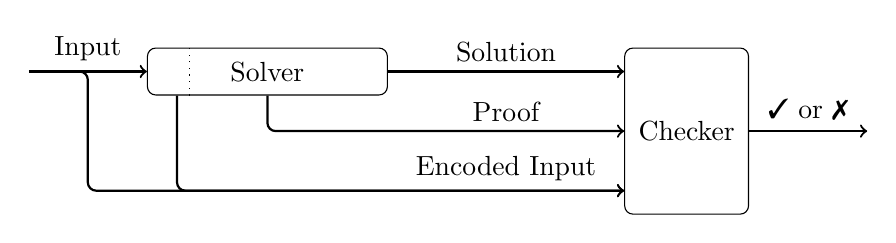
\begin{tikzpicture}
            \node (solver) [inner xsep=3em, inner ysep=0.5em, draw, rounded corners=3pt] { Solver };

            \node (checker) [right=3cm of solver.north east, anchor=north west,
            inner xsep=0.5em, draw, rounded corners=3pt, minimum height=6em, visible on=<3->] { Checker };

            \draw [->, thick] (solver.east) -- (solver.east -| checker.west)
                coordinate [midway] (solutionmid) node [above, midway] { Solution };

            \draw [->, thick, rounded corners=3pt, visible on=<2->] (solver.south) -- (solver.south |- checker.west)
                -- (checker.west) coordinate [midway] (proofmid);

            \coordinate (prooflabel) at (proofmid-|solutionmid);
            \node [above=0cm of prooflabel, visible on=<2->] { Proof };

            \coordinate [right=1.5cm of checker.east] (verified);
            \draw [->, thick, visible on=<5->] (checker.east) -- (verified) node [above, midway] { \ding{51} or \ding{55} };

            \coordinate [left=1.5cm of solver.west] (input);
            \draw [->, thick] (input) -- (solver.west) coordinate [midway] (inputmid) node [above, midway] { Input };

            \coordinate (checkerbotleft) at ($(checker.west)+($(checker.west)-(solver.east-|checker.west)$)$);

            \draw [->, thick, rounded corners=3pt, visible on=<3>] ($(inputmid)+(-0.2,0)$) --
            (inputmid) -- (inputmid |- checkerbotleft) -- (checkerbotleft) coordinate [midway] (altinputmid);
            \coordinate (solverstart) at ($(solver.south)!0.75!(solver.south west)$);
            \coordinate (solverstart2) at ($(solver.south)!0.65!(solver.south west)$);
            \draw [dotted, visible on=<4->] (solverstart2) -- (solverstart2 |- solver.north);
            \draw [->, thick, rounded corners=3pt, visible on=<4->] (solverstart) -- (solverstart |- checkerbotleft) -- (checkerbotleft);

            \coordinate (prooflabel) at (altinputmid-|solutionmid);
            \node [above=0cm of prooflabel, visible on=<4->] { Encoded Input };
        \end{tikzpicture}
    \end{center}

    \uncover<6->{
    \begin{itemize}
        \item Keep the compilation simple!
        \item For now: testing.
        \item Possible future direction: formally verified compilation.
    \end{itemize}}
\end{frame}

\begin{frame}[t]{Compiling CP Variables}
    Given $A \in \{ -3 \ldots 9 \}$:
\only<1>{
    \begin{align*}
        a_{{=}-3} + a_{{=}-2} + a_{{=}-1} + a_{{=}0} + a_{{=}1} + a_{{=}2}
        + a_{{=}3} \\ +~a_{{=}4} + a_{{=}5} + a_{{=}6} + a_{{=}7}
        + a_{{=}8} + a_{{=}9} &= 1
    \end{align*}
}\only<2->{
\begin{align*}
    -16 a_{{\operatorname{neg}}} + 1 a_{{\operatorname{b}}0} + 2 a_{{\operatorname{b}}1} + 4
    a_{{\operatorname{b}}2} + 8 a_{{\operatorname{b}}3} &\ge -3
    \textnormal{~and}\\
    16 a_{{\operatorname{neg}}} + -1 a_{{\operatorname{b}}0} + -2 a_{{\operatorname{b}}1} +
    -4 a_{{\operatorname{b}}2} + -8 a_{{\operatorname{b}}3} &\ge -9
\end{align*}

    \only<3->{
    Then where needed, define:
    \begin{align*}
        a_{{\ge}4} & \leftrightarrow -16 a_{{\operatorname{neg}}} + 1 a_{{\operatorname{b}}0} + 2 a_{{\operatorname{b}}1} + 4
        a_{{\operatorname{b}}2} + 8 a_{{\operatorname{b}}3} &\ge 4 \\
        a_{{\ge}5} & \leftrightarrow -16 a_{{\operatorname{neg}}} + 1 a_{{\operatorname{b}}0} + 2 a_{{\operatorname{b}}1} + 4
        a_{{\operatorname{b}}2} + 8 a_{{\operatorname{b}}3} &\ge 5 \\
        a_{{=}4} & \leftrightarrow a_{{\ge}4} \land \overline{a}_{{\ge}5}
    \end{align*}

    We can do this in the pseudo-Boolean model, where needed, or lazily inside
    the proof using extension variables.
}}
\end{frame}

\begin{frame}{Introducing Useful Facts About Variables}
    When creating $x_{{=}i}$, also introduce
    \begin{align*}
        x_{{\ge}i} \rightarrow x_{{\ge}j} \quad \text{and} \quad x_{{\ge}h} \rightarrow x_{{\ge}i}
    \end{align*}
    for the closest two values $h$ and $j$ that already have equality variables.

    \bigskip\pause

    All-different is easier if we introduce \begin{align*}
    \sum_{i=\ell}^{u} x_{{=}i} \ge 1
    \end{align*}
    which is also easy to do in a proof.
\end{frame}

\begin{frame}{Compiling Constraints}
    \only<1>{
        \begin{itemize}
            \item Also need to compile every constraint to pseudo-Boolean form.
            \item Doesn't need to be a propagating encoding.
            \item Can use additional variables.
        \end{itemize}
    }\only<2>{
    Given $2A + 3B + 4C \ge 42$, where $A, B, C \in \{ -3 \ldots 9 \}$,
\begin{align*}
    -32 a_{{\operatorname{neg}}} + 2 a_{{\operatorname{b}}0} + 4 a_{{\operatorname{b}}1} + 8
    a_{{\operatorname{b}}2} + 16 a_{{\operatorname{b}}3} \\
    + -48 b_{{\operatorname{neg}}} + 3 b_{{\operatorname{b}}0} + 6
    b_{{\operatorname{b}}1} + 12 b_{{\operatorname{b}}2} + 24 b_{{\operatorname{b}}3}\\
    + -64 c_{{\operatorname{neg}}} + 4 c_{{\operatorname{b}}0} + 8
    c_{{\operatorname{b}}1} + 16 c_{{\operatorname{b}}2} + 32 c_{{\operatorname{b}}3} & \ge 42 \textnormal{.}
\end{align*}}\only<3>{
    Given $(A, B, C) \in [(1, 2, 3), (1, 3, 4), (2, 2, 5)]$, define
    \begin{align*}
        3\overline{t}_{0} + a_{{=}1} + b_{{=}2} + c_{{=}3} \ge 3 &\quad \text{i.e.}&t_{0} \rightarrow (a_{{=}1} \wedge b_{{=}2} \wedge c_{{=}3}) \\
        3\overline{t}_{1} + a_{{=}1} + b_{{=}4} + c_{{=}4} \ge 3 &\quad \text{i.e.}&t_{1} \rightarrow (a_{{=}1} \wedge b_{{=}4} \wedge c_{{=}4}) \\
        3\overline{t}_{2} + a_{{=}2} + b_{{=}2} + c_{{=}5} \ge 3 &\quad \text{i.e.}&t_{2} \rightarrow (a_{{=}2} \wedge b_{{=}2} \wedge c_{{=}5})
    \end{align*} using a tuple selector variable \begin{align*}
        &t_{0} + t_{1} + t_{2} = 1
    \end{align*}}
\end{frame}

\begin{frame}{Proof Logging Search Trees}
    Want to just output a reverse unit propagation step on every backtrack.

    \bigskip

    This works for forward-checking / DPLL, but not with strong propagators.

    \bigskip

    The key invariant: any propagation visible to the CP solver must be reflected either
    \begin{itemize}
        \item By ``unit propagation'' on the pseudo-Boolean model,
        \item Or by reverse unit propagation on the backtrack clause.
    \end{itemize}
\end{frame}

\begin{frame}{Proof Logging Inference: The Easy Cases}
    If it follows from bounds consistency on the pseudo-Boolean model,
    no further proof logging needed.

    \bigskip

    For example, a tuple in a table constraint becoming infeasible.

    \bigskip

    Intuition: some facts are so obvious they don't need stated.
\end{frame}

\begin{frame}{Proof Logging Inference: Using RUP}
    Some facts are ``obvious'' once we tell the proof verifier they are true,
    but not otherwise.

    \bigskip

    For example, a variable losing a value due to a table constraint.

    \bigskip

    We log these propagations using RUP.

    \bigskip

    Intuition: like singleton arc consistency.
\end{frame}

\begin{frame}{Proof Logging Inference: Explicit Justifications}
    Some facts aren't ``obvious'' but can be justified explicitly.

    \bigskip

    All-different: sum up the ``variable takes at least one value'' and ``value is used at most once'' constraints for a Hall set or Hall violator.

    \bigskip

    Integer linear inequalities: the slack algorithm gives an easy proof.
\end{frame}

\begin{frame}[t]{Justifying All-Different Failures}
    \begin{tabular}{r@{\hspace*{0mm}}c@{\hspace*{0.6mm}}c@{\hspace*{0.6mm}}c@{\hspace{0.6mm}}c@{\hspace*{0.6mm}}r@{\hspace*{3mm}}r@{\hspace*{0.8mm}}r@{\hspace*{0.8mm}}r@{\hspace*{0.8mm}}r@{\hspace*{0.8mm}}r@{\hspace*{0.8mm}}r@{\hspace*{0.8mm}}r@{\hspace*{0.8mm}}r@{\hspace*{0.8mm}}r@{\hspace*{0.8mm}}l}
    $v \in \{$ &
    1 &
      &
      &
        4 \hspace*{1.2mm} 5 &
    $\}$ &
    &
    &
    &
    &
    &
    &
    &
    &
    &
    \\

        $\only<1>{w}\only<2->{{\color{uofgcobalt}w}} \in \{$ &
    1 &
    2 &
    3 &
        &
    $\}$ &
        $\only<1-2>{\phantom{w_{{=}1}}}\only<3->{w_{{=}1}}$ &
        $\only<1-2>{\phantom{+}}\only<3->{+}$ &
        $\only<1-2>{\phantom{w_{{=}2}}}\only<3->{w_{{=}2}}$ &
        $\only<1-2>{\phantom{+}}\only<3->{+}$ &
        $\only<1-2>{\phantom{w_{{=}3}}}\only<3->{w_{{=}3}}$ &
    &
    &
        &
        &
        $\only<1-2>{\phantom{ \ge 1}}\only<3->{ \ge 1}$
        \\

        $\only<1>{x}\only<2->{{\color{uofgcobalt}x}} \in \{$ &
    &
    2 &
    3 &
        &
    $\}$ &
        &
        &
        $\only<1-3>{\phantom{x_{{=}2}}}\only<4->{x_{{=}2}}$ &
        $\only<1-3>{\phantom{+}}\only<4->{+}$ &
        $\only<1-3>{\phantom{x_{{=}3}}}\only<4->{x_{{=}3}}$ &
        &
        &
        &
        &
        $\only<1-3>{\phantom{ \ge 1}}\only<4->{ \ge 1}$
        \\

        $\only<1>{y}\only<2->{{\color{uofgcobalt}y}} \in \{$ &
    1 &
    &
    3 &
        &
    $\}$ &
        $\only<1-3>{\phantom{y_{{=}1}}}\only<4->{y_{{=}1}}$ &
        &
        &
        $\only<1-3>{\phantom{+}}\only<4->{+}$ &
        $\only<1-3>{\phantom{y_{{=}3}}}\only<4->{y_{{=}3}}$ &
    &
    &
        &
        &
        $\only<1-3>{\phantom{ \ge 1}}\only<4->{ \ge 1}$
        \\

        $\only<1>{z}\only<2->{{\color{uofgcobalt}z}} \in \{$ &
    1 &
    &
    3 &
        &
    $\}$ &
        $\only<1-3>{\phantom{z_{{=}1}}}\only<4->{z_{{=}1}}$ &
        &
        &
        $\only<1-3>{\phantom{+}}\only<4->{+}$ &
        $\only<1-3>{\phantom{z_{{=}3}}}\only<4->{z_{{=}3}}$ &
    &
    &
        &
        &
        $\only<1-3>{\phantom{ \ge 1}}\only<4->{ \ge 1}$
        \\[0.5cm]

        \only<5->{
    &
    $\rightarrow$ &
    &
    &
    &
    &
    $-v_{{=}1}$ &
    $+$ &
    $-w_{{=}1}$ &
    $+$ &
    &
     &
    $-y_{{=}1}$ &
    $+$ &
    $-z_{{=}1}$ &
    $ \ge -1$ \\

    &
    &
    $\rightarrow$ &
    &
    &
    &
    &
    &
    $-w_{{=}2}$ &
    $+$ &
    $-x_{{=}2}$ &
     &
    &
     &
    &
    $ \ge -1$ \\

    &
    &
    &
    $\rightarrow$ &
    &
    &
    &
    &
    $-w_{{=}3}$ &
    $+$ &
    $-x_{{=}3}$ &
    $+$ &
    $-y_{{=}3}$ &
    $+$ &
    $-z_{{=}3}$ &
    $ \ge -1$
    \\[0.5cm]
}
\only<6->{
    &
    &
    &
    &
    &
    &
    $-v_{{=}1}$ &
     &
    &
    &
    &
     &
     &
     &
     &
    $ \ge 1$ \\
}
\only<7->{
    &
    &
    &
    &
    &
    &
    $ v_{{=}1}$ &
     &
    &
    &
    &
     &
     &
     &
     &
    $ \ge 0$ \\[0.5cm]
}
\only<8->{
    &
    &
    &
    &
    &
    &
    $0$ &
     &
    &
    &
    &
     &
     &
     &
     &
    $ \ge 1$ \\
}
    &
    $\phantom{\rightarrow}$ &
    $\phantom{\rightarrow}$ &
    $\phantom{\rightarrow}$ &
    &
    &
    $\phantom{-v_{{=}1}}$ &
    $\phantom{+}$ &
    $\phantom{-w_{{=}1}}$ &
    $\phantom{+}$ &
    $\phantom{-y_{{=}1}}$ &
    $\phantom{+}$ &
    $\phantom{-y_{{=}1}}$ &
    $\phantom{+}$ &
    $\phantom{-z_{{=}1}}$ &
    $\phantom{ \ge -1}$ \\
    \end{tabular}
\end{frame}

\begin{frame}{Proof Logging Reformulations}
    Some reformulations can be done inside the proof log.

    \bigskip

    We know how to do:
    \begin{itemize}
        \item Turning not-equals from sums into binary constraints.
        \item 2D element constraints.
        \item Autotabulation.
    \end{itemize}
\end{frame}

\begin{frame}{The Glasgow Constraint Solver}
    \begin{center}
        \raisebox{-0.3em}{\url{https://github.com/ciaranm/glasgow-constraint-solver}}
        \bigskip
    \end{center}
    \begin{itemize}
        \item MIT licence, written in fancy modern C++.
        \item All-different, integer linear inequality (including for variables
            with very large domains), table, minimum / maximum of an array,
            element, and absolute value.
        \item I couldn't think of a name.
    \end{itemize}
\end{frame}

\begin{frame}{Propagator Bugs!}
    \begin{itemize}
        \item Early versions of integer linear inequality propagator had bug with negative values and negative coefficients.
            \begin{itemize}
                \item Integer division and modulus in C++ don't do what you expect for negative numbers.
                \item I had forgotten this.
            \end{itemize}
        \item Using ``trust me'' assertions, no wrong answers from many tests.
        \item Using proof logging: caught instantly.
    \end{itemize}
\end{frame}

\begin{frame}{How Expensive is Proof Logging?}
    \only<1>{
        \begin{itemize}
            \item Laurent D. Michel, Pierre Schaus, Pascal Van Hentenryck:
                MiniCP: a lightweight solver for constraint programming. Math. Program. Comput.
                13(1) (2021).
            \item Five benchmark problems allowing comparison of solvers ``doing the same thing'':
                \begin{itemize}
                    \item Simple models.
                    \item Fixed search order and well-defined propagation consistency levels.
                    \item Few global constraints (although we don't have circuit yet).
                \end{itemize}
            \item Probably close to the worst case for proof logging performance.
            \item Also: Crystal Maze and World's Hardest Sudoku.
        \end{itemize}
    }\only<2>{
        \begin{itemize}
            \item Our solver: faster than the fastest of MiniCP, OscaR, and Choco.
            \item Proof logging slowdown: between 8.4 to 61.1.
                \begin{itemize}
                    \item 800,000 to 3,000,000 inferences per second.
                    \item Proof logs can be hundreds of GBytes.
                    \item No effort put into making the proof-writing code run fast.
                \end{itemize}
            \item Verification slowdown: a further 10 to 100.
                \begin{itemize}
                    \item Probably possible to reduce this substantially if we are prepared to put more care into writing proofs.
                \end{itemize}
        \end{itemize}}
\end{frame}

\begin{frame}{What Do We Have?}
    \begin{itemize}
        \item Don't know that the solver is correct.
        \item Do know that if a solver ever produces a wrong answer, it can be detected.
            \begin{itemize}
                \item Even if due to a hardware or compiler error, or faulty maths.
                \item We will need to get used to verification being (a constant factor) slower than solving.\pause
                \item Under the assumption that the pseudo-Boolean problem is correct.
            \end{itemize} \pause
        \item Also helps with testing and solver development: bugs are caught if incorrect reasoning is performed,
            rather than if a wrong answer is produced. \pause
        \item We get an auditable record of exactly what was actually solved. \pause
        \item Potentially possible to re-use proof logs for empirical algorithmics?
    \end{itemize}
\end{frame}

{
    \usebackgroundtemplate{
        \tikz[overlay, remember picture]
        \node[at=(current page.south), anchor=south, inner
        sep=0pt]{\includegraphics[keepaspectratio=true, width=\paperwidth]{background4.jpg}};
    }

    \begin{frame}[plain,noframenumbering]
        \begin{tikzpicture}[remember picture, overlay]
            \node at (current page.north west) {
                \begin{tikzpicture}[remember picture, overlay]
                    \fill [fill=uofguniversityblue, anchor=north west] (0, 0) rectangle (\paperwidth, -2.8cm);
                \end{tikzpicture}
            };

            \node (logo) [anchor=north east, shift={(-0.6cm,-0.2cm)}] at (current page.north east) {
                
\includegraphics[keepaspectratio=true,scale=0.5]{UoG_keyline.pdf}
            };

            \node (logo2) [anchor=north, below=0.2cm of logo.south] {
                
\includegraphics[keepaspectratio=true,scale=0.1]{RAEngWhite.pdf}
            };

            \coordinate (logos) at ($(logo.south)!0.5!(logo2.north)$);

            \node [anchor=west, xshift=0.2cm] at (current page.west |- logos) {
                \begin{minipage}{0.60\paperwidth}\raggedright
                    \textcolor{white}{\url{https://ciaranm.github.io/}} \\[0.3cm]
                    \textcolor{white}{\href{mailto:ciaran.mccreesh@glasgow.ac.uk}{\nolinkurl{ciaran.mccreesh@glasgow.ac.uk}}}
                \end{minipage}
            };
        \end{tikzpicture}
    \end{frame}
}

\end{document}
